\documentclass[red]{beamer}
% Class options include: notes, notesonly, handout, trans,
%                        hidesubsections, shadesubsections,
%                        inrow, blue, red, grey, brown


% Theme for beamer presentation.
\usepackage{beamerthemetree} 
% Other themes include: beamerthemebars, beamerthemelined, 
%                       beamerthemetree, beamerthemetreebars  
\usepackage{listings}

\title{ImpactJS Presentation}    
\author{David Leonard}                 
\institute{City College of New York}      
\date{\today}                   

\begin{document}

\lstdefinelanguage{JavaScript}{
  keywords={typeof, new, true, false, catch, function, return, null, catch, switch, var, if, in, while, do, else, case, break, this},
  keywordstyle=\color{blue}\bfseries,
  ndkeywords={class, export, boolean, throw, implements, import, this},
  ndkeywordstyle=\color{darkgray}\bfseries,
  identifierstyle=\color{black},
  sensitive=false,
  comment=[l]{//},
  morecomment=[s]{/*}{*/},
  commentstyle=\color{purple}\ttfamily,
  stringstyle=\color{red}\ttfamily,
  morestring=[b]',
  morestring=[b]"
}

\lstset{
   language=JavaScript,
   extendedchars=true,
   basicstyle=\scriptsize\ttfamily,
   showstringspaces=false,
   showspaces=false,
   tabsize=2,
   breaklines=true,
   showtabs=false,
   captionpos=b
}

% Object code listing
\defverbatim[colored]\lstI{
	\begin{lstlisting}
		var person = {
			name: David,
			age: 23,
			major: Computer Science
		};
		
		person.name; // David
		person.age; // 23
		person.major; // Computer Science 
	\end{lstlisting}
}

% Init function code listing
\defverbatim[colored]\lstll{
	\begin{lstlisting}
	init: function(){
		// Init function is only run once 
		ig.input.bind( ig.KEY.LEFT_ARROW, 'left');
		ig.input.bind( ig.KEY.RIGHT_ARROW, 'right');
		ig.input.bind( ig.KEY.X, 'jump');
	}
	\end{lstlisting}
}

% Update function code listing
\defverbatim[colored]\lstlll{
	\begin{lstlisting}
	update: function(){
		// update is run once per frame
		if( typeof player === undefined ){
			var player = this.getEntitiesByType(EntityPlayer)[0];
			this.screen.x = player.pos.x - ig.system.width/2;
			this.screen.y = player.pos.y - ig.system.height/2;
		}
	}
	\end{lstlisting}
}

% Draw function code listing
\defverbatim[colored]\lstllll{
	\begin{lstlisting}
	draw: function(){
		this.parent();
		if(this.font){
			var player = this.getEntitiesByType(EntityPlayer)[0];
			this.font.draw('Health: ' + player.health, 50, 10, ig.Font.ALIGN.CENTER);
		}
	}
	\end{lstlisting}
}

% Main.js module loading
\defverbatim[colored]\lstlllll{
    \begin{lstlisting}
        ig.module(
            'game.main'
        )
        .requires(
            'impact.game',
            'impact.debug.debug',
            'game.levels.test',
            'game.entities.player',
            'game.entities.goomba'
        )
    \end{lstlisting}
}

% main.js .defines
\defverbatim[colored]\lstllllll{
    \begin{lstlisting}
        .defines(function(){
            MyGame = ig.Game.extend({

            });

            ig.main( '#canvas', MyGame, 60, 320, 240, 2 );
            });
        });
    \end{lstlisting}
}

% main.js properties
\defverbatim[colored]\lstlllllll{
    \begin{lstlisting}
        .defines(function(){
            MyGame = ig.Game.extend({
                font: new ig.Font('media/04b03.font.png'),
                gravity: 300,
            });

            [ ... ]
        });
    \end{lstlisting}
}

% main.js init function
\defverbatim[colored]\lstllllllll{
    \begin{lstlisting}
    MyGame = ig.Game.extend({
        init: function(){
            ig.input.bind( ig.KEY.LEFT_ARROW, 'left');
            ig.input.bind( ig.KEY.RIGHT_ARROW, 'right');
            ig.input.bind( ig.KEY.X, 'jump');
            this.loadLevel( LevelTest );
        }
    });
    \end{lstlisting}
}

% main.js update function
\defverbatim[colored]\lstlllllllll{
    \begin{lstlisting}
    MyGame = ig.Game.extend({
        init: [ ... ],

        update: function(){
            var player = this.getEntitiesByType( EntityPlayer )[0];
            if( player ) {
            this.screen.x = player.pos.x - ig.system.width/2;
            this.screen.y = player.pos.y - ig.system.height/2;
            }
            this.parent();
        },
    });

    \end{lstlisting}
}

% main.js draw function
\defverbatim[colored]\lstllllllllll{
    \begin{lstlisting}
    MyGame = ig.Game.extend({
        update: [ ... ],
        draw: function(){
            this.parent();
            if(this.font){
                var player = ig.game.getEntitiesByType('EntityPlayer')[0];
                this.font.draw('Health: ' + player.health, 50, 10, ig.Font.ALIGN.CENTER);
            }
        },
    });
    \end{lstlisting}
}

% player.js module
\defverbatim[colored]\lstlllllllllll{
    \begin{lstlisting}
    ig.module(
        'game.entities.player'
    )
    .requires(
        'impact.entity'
    )
    .defines(function(){
        EntityPlayer = ig.Entity.extend({

        });

    });
    \end{lstlisting}   
}


% player.js properties (collision)
\defverbatim[colored]\lstllllllllllll{
    \begin{lstlisting}
    EntityPlayer = ig.Entity.extend({
        type: ig.Entity.TYPE.A,
        checkAgainst: ig.Entity.TYPE.NONE,
        collides: ig.Entity.COLLIDES.ACTIVE,
    });
    \end{lstlisting}
}

% player.js physics properties
\defverbatim[colored]\lstlllllllllllll{
    \begin{lstlisting}
    EntityPlayer = ig.Entity.extend({
        [ ... ],
        animSheet: new ig.AnimationSheet('media/player.png', 16, 28),
        size: {x: 16, y: 28},
        offset: {x: 1, y: 0},
        flip: true,
        maxVel: {x: 100, y: 160},
        friction: {x: 500, y: 0},
        accelGround: 200,
        accelAir: 310,
        jump: 360,
        gravity: 300,
    });
    \end{lstlisting}
}

% player.js init function
\defverbatim[colored]\lstllllllllllllll{
    \begin{lstlisting}
    EntityPlayer = ig.Entity.extend({
        [ ... properties ...],

        init: function(x, y, settings){
            this.parent(x, y, settings);
            this.addAnim('idle', 1, [1]);
            this.addAnim('run', 0.10, [1, 0]);
            this.addAnim('jump', 1, [2]);
            this.addAnim('fall', 0.4, [2]);
        },
    });
    \end{lstlisting}
}

% player.js update function (part 1)
\defverbatim[colored]\lstlllllllllllllll{
    \begin{lstlisting}
    [ ... properties ... ]
    init: [ ... ]
    update: function(){
        // Add left/right/jump movement logic
        var accel = this.standing ? this.accelGround : this.accelAir;
        if(ig.input.state('left')) {
            this.accel.x = -accel;
            this.flip = false;
        } else if(ig.input.state('right')) {
            this.accel.x = accel;
            this.flip = true;
        } else
            this.accel.x = 0;
    },
    \end{lstlisting}
}

% player.js update function (part 2)
\defverbatim[colored]\lstllllllllllllllll{
    \begin{lstlisting}
    update: function(){
        [ ... ]
        if(this.standing && ig.input.state('jump')) {
            if(this.vel.y == 0) {
                this.vel.y = -this.jump;
                this.falling = false;
            }
        }

        // CASE 2: Player not standing, jump has been released and we're not falling
        // we reduce the y velocity by 66% and mark us as falling
        else if(!this.standing && !ig.input.state('jump') && !this.falling) {
            this.vel.y = Math.floor(this.vel.y/3);
            this.falling = true;
        }
    },
    \end{lstlisting}
}

% player.js update function (part 3)
\defverbatim[colored]\lstlllllllllllllllll{
    \begin{lstlisting}
    update: function(){
        [ ... ]

        // Add moving logic
        this.currentAnim.flip.x = this.flip;
        this.parent();

        if(this.vel.y < 0 && !this.standing)
            this.currentAnim = this.anims.jump;
        else if(this.vel.y > 0 && !this.standing)
            this.currentAnim = this.anims.fall;
        else if(this.vel.x != 0)
            this.currentAnim = this.anims.run;
        else
            this.currentAnim = this.anims.idle;
    },
    \end{lstlisting}
}


% Creates title page of slide show using above information
\begin{frame}
  \titlepage
\end{frame}

\section[Outline]{}

\section{ImpactJS and JavaScript Introduction}

\begin{frame}
    \frametitle{What is a game engine?}
    \begin{itemize}
        \item<1-> Just a collection of algorithms
        \item<2-> Exposes functionality for use
        \item<3-> Not a point and click tool
    \end{itemize}
\end{frame}

\begin{frame}
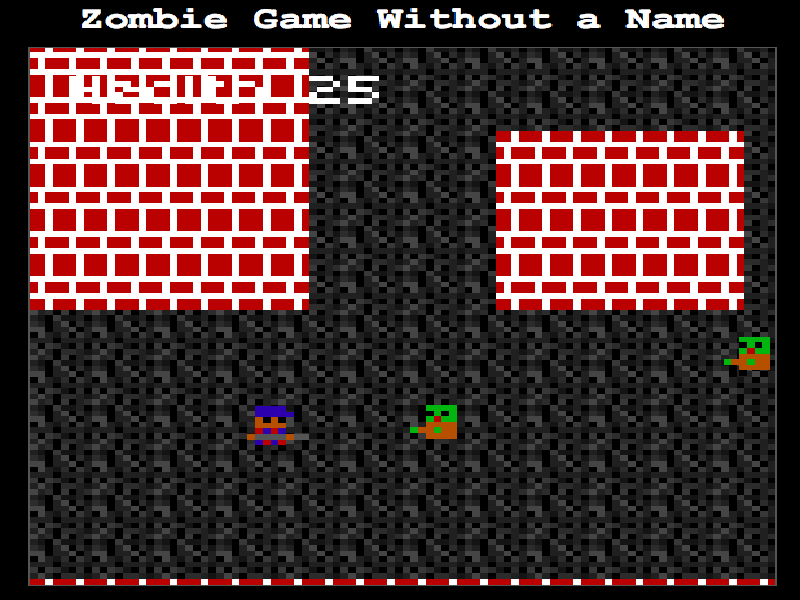
\includegraphics[height=0.9\textheight]{zombie.png}
\end{frame}

\begin{frame}
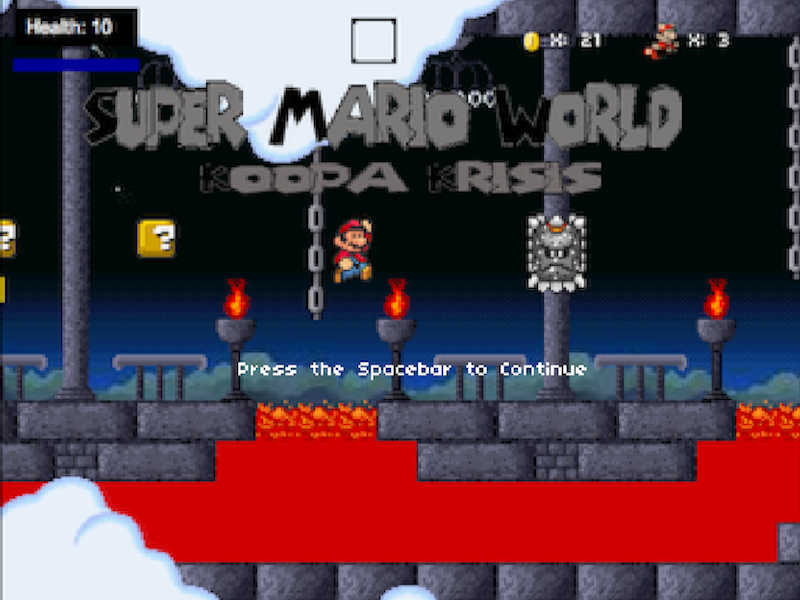
\includegraphics[height=0.9\textheight]{titlescreen.png}
\end{frame}

\begin{frame}
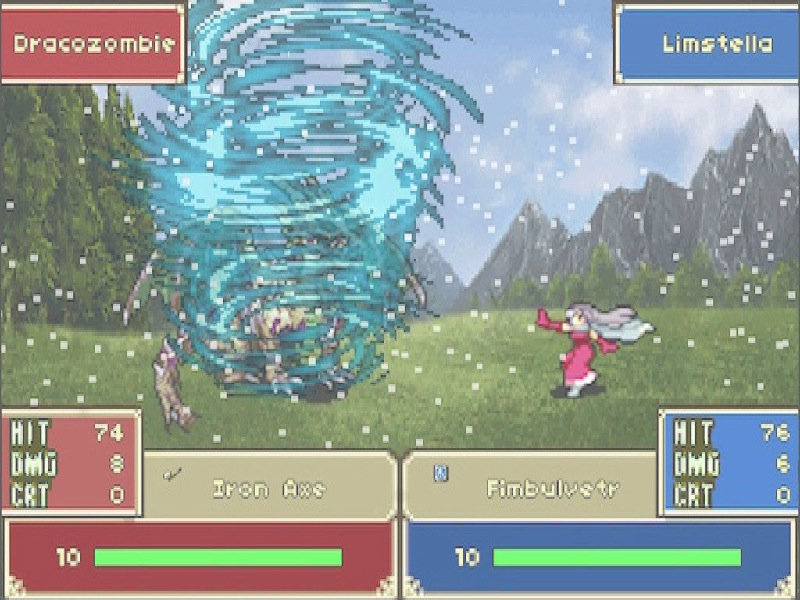
\includegraphics[height=0.9\textheight]{fireemblem.jpg}
\end{frame}

\subsection{ImpactJS Strengths}

\begin{frame}
  \frametitle{Why ImpactJS?}   % Insert frame title between curly braces

  \begin{itemize}
  \item Collision handling
  \item Camera pluginss
  \item Map Editor
  \item Player Physics
  \item Strong OOP Design
  \end{itemize}
\end{frame}

\subsection{JavaScript Types}

\begin{frame}
	\frametitle{JavaScript Types}
	 \begin{itemize}
  		\item<1-> strings : "Hello World"
 		\item<2-> number : var x = 45
 		\item<3-> boolean : var flip = true
		\item<4-> function
		\item<4-> array : var arr = [ 1, 2, 3, 4 ]
		\item<5->object : person = \{ name: David, Age: 23 \}
		\item<6->undefined : typeof person === undefined
		\item<7->null : var x = null
 	 \end{itemize}
\end{frame}

\begin{frame}
 	\frametitle{JavaScript Objects}
		\lstI
\end{frame}

\section{Understanding ImpactJS Game Loop}


\section{Starting your first game}
\subsection{main.js}
\begin{frame}
    \frametitle{main.js}
    \begin{itemize}
        \item<1-> Require all modules
        \item<2-> Define game classes
        \item<3-> Bind keys within Init()
        \item<4-> Camera code, game logic within Update()
        \item<5-> Draw images within Draw()
    \end{itemize}
\end{frame}


\end{document}
